% This is samplepaper.tex, a sample chapter demonstrating the
% LLNCS macro package for Springer Computer Science proceedings;
% Version 2.21 of 2022/01/12
%
\documentclass[runningheads]{llncs}
%
\usepackage[T1]{fontenc}
% T1 fonts will be used to generate the final print and online PDFs,
% so please use T1 fonts in your manuscript whenever possible.
% Other font encondings may result in incorrect characters.
%
\usepackage{graphicx}
\usepackage{amsmath}
\usepackage{booktabs,multicol,multirow,tabularx,array}          % Packages para tabela
\usepackage{cite}
\usepackage{makecell}
\usepackage{hyperref}
% Used for displaying a sample figure. If possible, figure files should
% be included in EPS format.
%
% If you use the hyperref package, please uncomment the following two lines
% to display URLs in blue roman font according to Springer's eBook style:
%\usepackage{color}
%\renewcommand\UrlFont{\color{blue}\rmfamily}
%\urlstyle{rm}
%
\begin{document}
%
\title{Human-Computer Interaction approach with Empathic Conversational Agent and Computer Vision}
%
\titlerunning{HCI approach with Empathic Conversational Agent and Computer Vision}
% If the paper title is too long for the running head, you can set
% an abbreviated paper title here
%
\author{Rafael Pereira\inst{1}\orcidID{0000-0001-8313-7253} \and
Carla Mendes\inst{1}\orcidID{0000-0001-7138-7124} \and
José Ribeiro\inst{1}\orcidID{0000-0003-3019-1330} \and
Nuno Rodrigues\inst{1}\orcidID{0000-0001-9536-1017} \and
António Pereira\inst{1,2}\orcidID{0000-0001-5062-1241}}
%
\authorrunning{Pereira, R et al.}
% First names are abbreviated in the running head.
% If there are more than two authors, 'et al.' is used.
%
\institute{Computer Science and Communications Research Centre, School of Technology and Management, Polytechnic of Leiria, 2411-901 Leiria, Portugal \\ \email{\{rafael.m.pereira, carla.c.mendes, jose.ribeiro, nunorod, apereira\}@ipleiria.pt} \and
INOV INESC Inovação, Institute of New Technologies, Leiria Office, 2411-901 Leiria, Portugal\\}

%
\maketitle              % typeset the header of the contribution
%
\begin{abstract}

The integration of empathy in Human-Computer Interaction (HCI) is essential for enhancing user experiences. Current HCI systems often overlook users' emotional states, limiting interaction quality. This research examines the integration of Multimodal Emotion Recognition (MER) into empathic generative-based conversational agents, encompassing facial, body, and speech emotion recognition, along with sentiment analysis. These elements are fused and incorporated into Large Language Models (LLMs) to continuously comprehend and respond to user empathically. This paper highlights the advantages of this multimodal approach over traditional unimodal systems in recognizing complex human emotions. Additionally, it provides a well-structured background on the addressed topics. The findings include a comprehensive guide on the impact of deep learning in HCI, a literature review on Emotion Recognition (ER) and conversational agents, and the proposal of an HCI architecture integrating MER with an empathic conversational agent. This research contributes significantly to the field of HCI by providing a detailed roadmap for developing more realistic and meaningful human-computer interactions.

\keywords{Human-Computer Interaction  \and Multimodal Emotion Recognition \and Fusion methods \and Empathic Conversational Agents}
\end{abstract}
%
%
%

\section{Introduction}

The concept of empathy consists of comprehending and sharing others' emotions to forge emotional connections, which is vital for human relationships. Similarly, in HCI, empathy is crucial in ensuring more realistic, improved, convenient and meaningful interactions. However, the typical HCI, aimed at tailoring computer systems to meet the specific needs and preferences of individuals, still lacks the users' emotional state, therefore losing crucial information during these interactions \cite{jaiswal_facial_2020}.  Recent Artificial Intelligence (AI) techniques, such as ER and empathic conversational agents, when integrated with HCI allow for continuous understanding of the user's emotions throughout interactions and empathically responding \cite{santos_approaches_2018}.

AI encompasses several techniques and methodologies aimed at enabling machines to perform tasks that typically require human intelligence, whereas deep learning stands out as an approach to processing unstructured data (including images, voice, videos, and text, among others) relying on Artificial Neural Networks (ANNs). ER, being a recent application of deep learning, involves detecting human emotions, generally through singular modalities such as facial features, gestures, poses, speech, and text captured through continuous interactions with the user \cite{alrowais_modified_2023}. On the other hand, generative-based conversational agents are designed to simulate human-like conversation and engage in interactions with users through natural language using several techniques, including Natural Language Processing (NLP), and deep learning with the recent advances in LLMs, to understand user input, interpret context, and generate appropriate responses.

Due to the advances of MER and conversational agents, individually, and the benefits provided when integrated with HCI, this study offers a guide covering ER modalities and key design and functionality aspects of a conversational agent. Lastly, proposing an HCI approach to ensure more realistic and meaningful interactions by leveraging HCI in conjunction with an emotion-branched fusion technique and an empathic conversational agent.
 
The main contributions of this study can be summarized as follows:
\begin{itemize}
	\item Detailed guide on how deep learning impacts HCI nowadays;
	\item Performed a background review regarding ER, fusion methods, and conversational agents;
	\item  Proposal of an HCI architecture approach aided with MER, through facial, body, and speech emotion recognition, sentiment analysis fused into an emphatic conversational agent powered with a LLM.
\end{itemize}

This research is divided into three sections. Section \ref{sec:background} presents the main concepts behind deep learning, ER, and conversational agents. Section \ref{sec:solution} shows the architecture, features, and characteristics of the proposed solution for HCI aided with ER fed into an empathic conversational agent. Lastly, Section \ref{sec:conclusions}  introduces the challenges and directions for future work and the conclusions. 

\section{Background}
\label{sec:background}

The evolution of technology in HCI has been significantly influenced by deep learning, a subset of machine learning. Deep learning has enhanced performance in domains such as speech recognition and object detection, with a focus on supervised learning. Supervised learning involves training a system with a labeled dataset to map inputs to outputs. The quality of training data is crucial for model efficacy, and techniques like data augmentation help in improving data diversity for better training outcomes \cite{Alrowais2023,Lecun2015}.

Convolutional Neural Networks (CNNs) are widely used for image-based tasks in HCI. These networks, with their structure of convolutional and pooling layers, process multi-array data like images efficiently, as depicted in Figure \ref{fig:cnnarchitecture}. This architecture is instrumental in emotion detection through computer vision, impacting HCI. CNNs not only enhance computational efficiency but also improve the robustness of the features extracted. Transfer learning plays a significant role in this context, facilitating knowledge transfer from large datasets to specific tasks and reducing the need for extensive data and computational resources \cite{Lecun2015, Khan2020}.

\begin{figure}[htb]
\centering
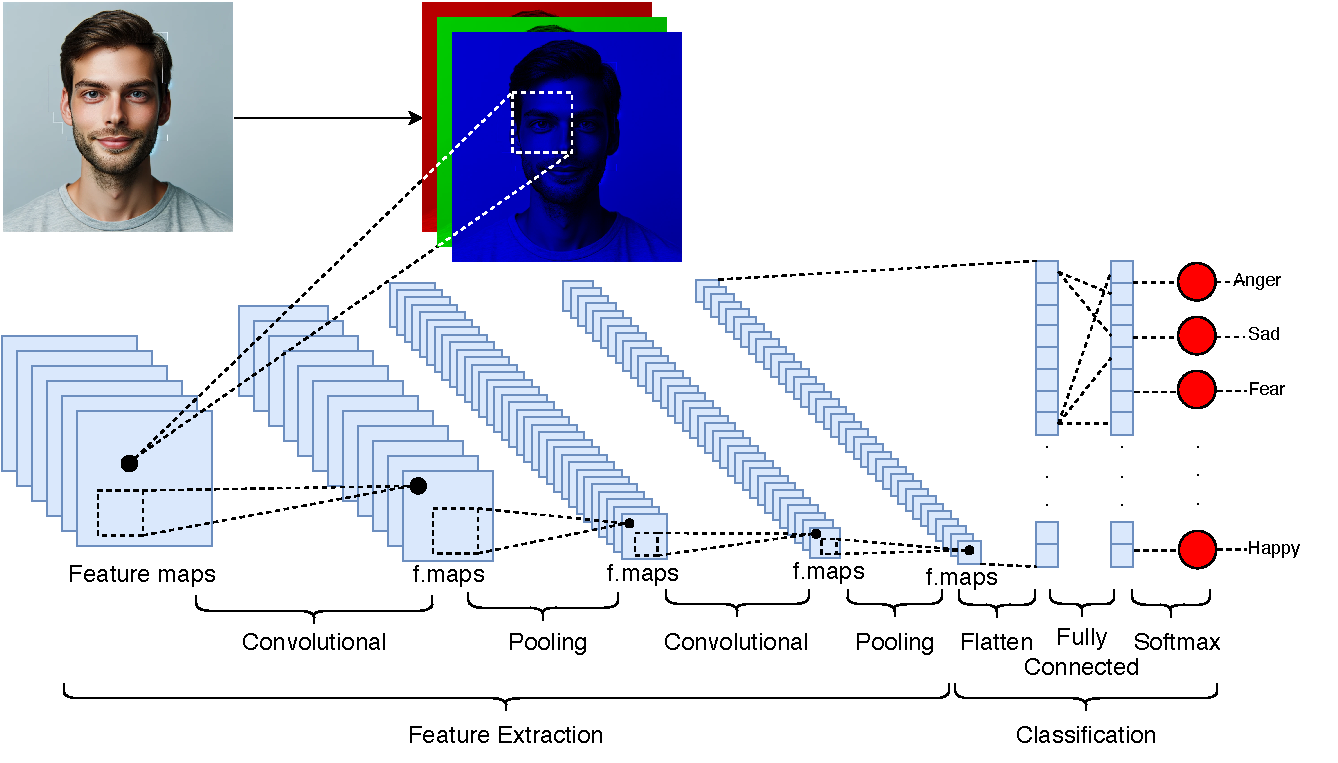
\includegraphics[width=0.97\linewidth]{CNNArchitecture.pdf}
\caption{An illustrative diagram of a CNN for emotion detection. The process begins with an input image of a smiling person and progresses through successive convolution and pooling layers for feature extraction. After flattening the feature maps, a fully connected network follows, leading to a final classification layer that categorizes the detected emotions into anger, sadness, fear, and happiness.}
\label{fig:cnnarchitecture}
\end{figure}

ER, related to analyzing human expressions and classifying them into emotions, is often studied individually and encounters challenges in real-life scenarios. This paper addresses these challenges through a multi-modal approach to emotion detection, aiming to mitigate problems associated with individual analysis methods. In computer vision, it includes facial movements and body language analysis from images and videos. On the other hand, linguistic contexts imply the usage of vocal nuances and text analysis to detect emotions \cite{Chul2018, Trigeorgis2016, Karna2020}. 

To achieve an aggregated emotion based on the four contexts described before, a fusion method could be employed which integrates information from these modalities by creating a single vector. These methods are categorized into early fusion, late fusion, and cross-modality fusion based on when the fusion process takes place \cite{sleeman_multimodal_2022, zhu_multimodal_2023}. Early fusion occurs before the application of primary learning models, consolidating all multimodal data (e.g. by concatenating incoming modality data) into a single representation. Early fusion is preferable when there exists a strong association between each data source. Late fusion, or decision-level fusion, involves applying the fusion model after the learning models, merging the outputs of each learning model (e.g. learned features or class probabilities) to produce a final classification. Late fusion is more effective in scenarios where each modality needs to be trained with a specific algorithm and when modalities are subject to volatility. Cross-modality fusion facilitates the exchange of modality-specific data either before or during the primary learning stage. This approach enables each modality to leverage the context provided by others, enhancing the predictive capabilities of the overall model \cite{sleeman_multimodal_2022}.

In the context of HCI, conversational agents are really important by interacting with users through simulated voice and/or text messages. These agents can either be domain-specific or versatile in handling various interaction types. The effectiveness of conversational agents largely depends on their response delivery mechanisms, which include rule-based, retrieval-based, and generative-based approaches. Each approach has its unique implementation complexity and response generation capability \cite{fernandes_survey_2020, ramesh_survey_2017}.

As a type of generative-based conversational agent, LLMs are sophisticated algorithms designed to produce human-like language in response to prompts. They leverage vast amounts of text data and employ techniques like unsupervised learning to understand the statistical patterns of language. Through the state-of-the-art pipeline stages of pretraining, supervised fine-tuning, reward modeling, and reinforcement learning, LLMs excel in capturing intricate linguistic patterns, nuances, and semantic relationships with the aid of transformer networks. LLMs utilize complex algorithms such as Variational Autoencoders (VAEs), Generative Adversarial Networks (GANs), or autoregressive models to create new textual content mirroring the characteristics of the training data. Among the popular LLMs are ChatGPT, LLaMA, Bard, Falcon, and others \cite{Hai_LLM_2023}. LLMs, although powerful, usually are computationally intensive due to the architecture and the size of the pre-trained parameters (often surpassing billions of parameters), bringing the need for a finetuning approach that reduces memory usage, number of parameters, and improves performance such as QLoRA which reduces the average memory requirements of finetuning  LLaMA 65B parameter model from >780GB of GPU memory to <48GB without degrading the runtime or predictive performance \cite{dettmers_qlora_2023}. Similarly, LoRa reduces the number of trainable parameters by 10,000 times and GPU memory requirement by 3 times (compared to GPT-3 175B) \cite{hu_lora_2021}.

\section{Proposed solution}
\label{sec:solution}

% Introduction of the proposed  solution:
% 	[X] - Briefly restate the problem your solution aims to solve.
% 	[X] - Introduce your multi-modal deep learning approach, emphasizing its novelty and potential benefits.
% It's missing we emphasise the novelty and the potential benefits
Empathy is a fundamental trait in ensuring realistic, natural, and meaningful interactions, therefore in the context of HCI, the goal is to provide authentic and engaging interactions through the use of empathic conversational agents. The architecture proposed in this paper, as depicted in Figure \ref{fig:approachArchitecture}, is an integrated system designed to enhance these interactions. Previous approaches in ER have often been unimodal, isolating text or facial features, despite the inherently complex and multimodal nature of human emotional expression, which encompasses verbal and non-verbal cues such as voice, behavior, and physiological signals \cite{ezzameli_emotion_2023, zhu_multimodal_2023}. The proposed architecture addresses this complexity with a dual-component system: a conversational agent module that maintains an ongoing interaction with the user, and a MER module. This latter module employs deep learning algorithms to analyze multiple data streams (textual, auditory, and visual), in unison, improving the accuracy and robustness of emotion detection. The fusion model within this system synergizes the different modalities, enhancing the strengths and balancing the limitations of each. Therefore, an implementation of this architecture tries to achieve a more nuanced, empathic conversational experience that aligns closely with human communication, which inherently weaves together speech, text, and visual information.

\begin{figure}[htb]
	\centering
	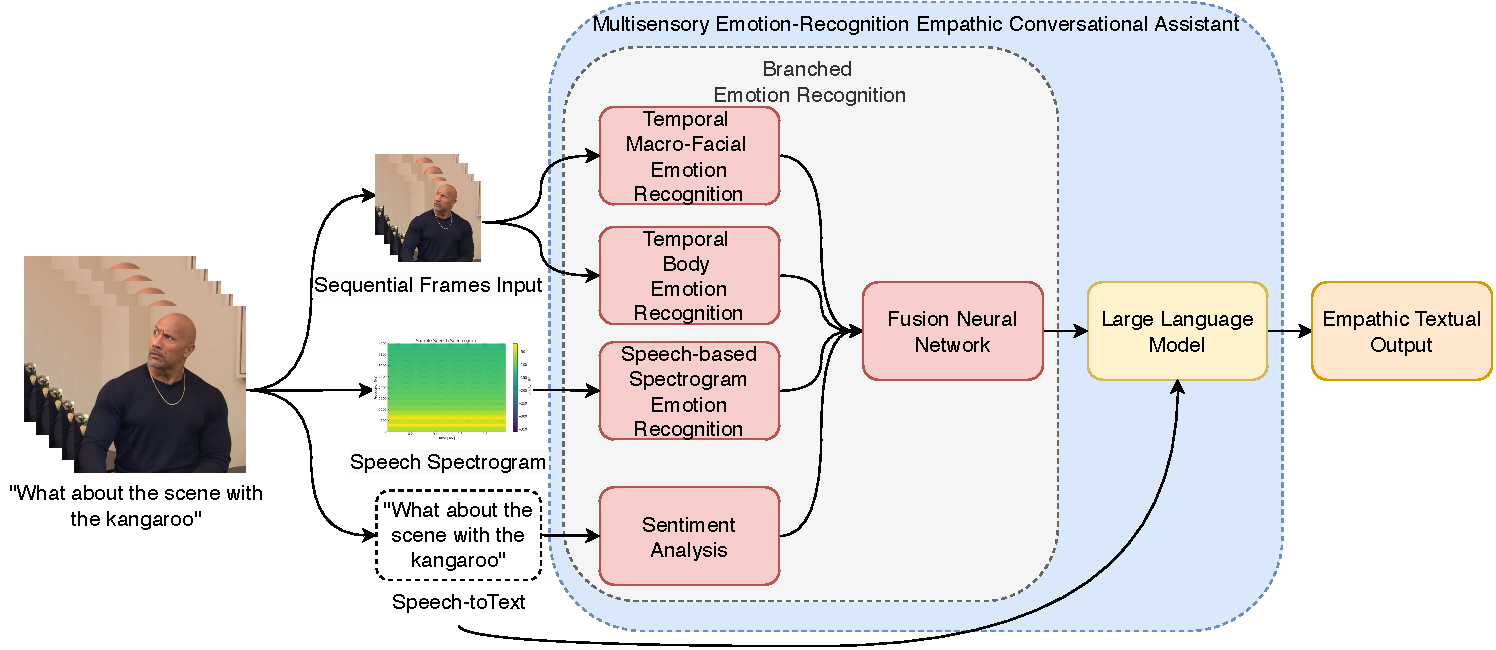
\includegraphics[width=0.97\linewidth]{approachArchitecture.pdf}
	\caption{Schematic representation of the proposed HCI approach architecture. Illustrates the flow from multimodal input through sequential frames, speech spectrograms, and text to the empathic conversational agent. The process integrates temporal macro-facial and body ER through computer vision, speech-based spectrogram ER, and sentiment analysis, leading to an empathic textual output generated by the fusion neural network and LLM.}
	\label{fig:approachArchitecture}
\end{figure}

% Overview of the Multi-modal System:
% 	[-] - Describe the overall architecture of your system.
% 		Here we could address where the data could be gathered from (real-time video and audio input, video data, both in a context of a conversational agent).
%		The visual data is composed by several frames, which serves as input in the Temporal Macro-Facial Emotion Recognition, and Temporal Body Emotion Recognition neural networks.
% 	[-] - Explain how it integrates different modalities (speech spectrogram, transcribed text, facial and body information) for emotion detection.
%		It would be nice to emphasise deeply that we want to gather the spectrogram from the speech, that we are detecting Macro-Facial Emotions, that its needed to perform a Speech-to-Text and then sentiment analysis.
%		It's necessary to normalise which emotions will be detected, and only in the implementation phase can be addressed.
%		The Fusion NN will return a single emotion, from the aggregation of the four NNs context-based emotion results.

% SA & SER
As previously detailed, the system could gather the visual and speech or textual data resulting from either in real-time or in video. Hence, the MER module analyzes in parallel all the present modalities, starting with textual data being analyzed by an sentiment analysis model to obtain the sentiment conveyed in the textual input, following preprocessing, feature extraction, and classification done with a 1D CNN classifier \cite{hung_beyond_2023}. On the other hand, the speech input can be firstly transcribed with automatic speech recognition algorithms, namely HMM-SVM hybrid model \cite{malik_automatic_2021}, to be passed on to the sentiment analysis model as text, while also being analyzed by the SER module composed of a CNN that analyzes the speech spectrogram (which represents the strength or loudness of a signal over time at different frequencies in a particular waveform) to extract the emotion conveyed in the speech \cite{Badshah2017}.

% FER e BER (In BER context, there's no guarantee of the presence of the whole body in every input (dataset, and in real-life environment), so the predictions could vary based on that.)
% In the context of FER and BER could be used only the facial and body landmarks (as a sequence, because of the temporal information). Or the whole frames information using, with a more complex and heavy but with excellent result NN.
% In both NN shall be present a LSTM layer, or ViT layer.
On the other hand, the visual data, obtained from computer vision, the user's macro-facial expressions and body pose are passed on to a Facial Emotion Recognition (FER) network and Body Emotion Recognition (BER) to further extract the emotional data conveyed in both input types.

The approach for the FER branch is to utilize advanced methods for precise detection and analysis of facial expressions. This includes the use of R-CNN for Region of Interest (ROI) detection and CNN for classification, as proposed by Zaman et al.~\cite{Zaman2022}. Another significant advancement is the use of transformers, specifically the FTCSAT model by Yao et al.~\cite{Yao2023}, to tackle challenges like low light conditions and variable head poses. The application of enhanced feature extraction techniques, as demonstrated by Sivaiah et al.~\cite{Bellamkonda2020}, and the integration of HOG descriptors with CNNs for classification further enrich this domain. Additionally, the incorporation of temporal layers, as explored by Mukhiddinov et al.~\cite{Mukhiddinov2023} in their two-branch CNN model, is relevant for the temporal context-aware of facial expressions. Fine-tuning pre-trained models is also a key strategy, enhancing the adaptability of FER systems to specific datasets or tasks.

The focus of BER branch is to analyze nonverbal cues such as posture and gestures through deep learning methods. Romeo et al.~\cite{Romeo2021} explore classification methods like 3D CNN and CNN + LSTM for gesture recognition, emphasizing the significance of temporal perception. Ilyas et al.~\cite{Ilyas2021} propose a method that combines the features of both facial and body gestures, using CNNs for feature extraction and LSTM for processing sequential information. The multimodal approach, as demonstrated by Hiranmayi et al.~\cite{Ranganathan2016}, is significant in achieving high accuracy in ER. Furthermore, the integration of a pre-trained VIT for gesture detection with a Resnet-34 model for facial macro-expression recognition, as done by Prakash et al.~\cite{Prakash2023}, showcases the potential of BER in complex scenarios like emotion detection in children with autism.

The final stage to obtain the final emotion prediction involves employing a late fusion model (using a neural network followed by a softmax layer as the final classifier), where the outputs (an array of emotion predictions) of the previously described models are combined, leveraging the strengths of each modality while compensating for their weaknesses. Hence, in some instances prioritizing certain modality data over the others. Late fusion models are advantageous over single modality models, which often struggle to generalize across diverse scenarios and may be sensitive to modality-specific noise. In contrast, late fusion models increase robustness to noise and variability, resulting in more reliable ER across situations and improved performance \cite{zhu_multimodal_2023, sleeman_multimodal_2022}. Therefore, the fusion model's output would consist of a single emotion resulting from the aggregation of the four context-based emotions obtained from each of the models. This approach benefits from the ability to train each modality with a specific algorithm and may make it easier to add or exchange different modalities in the future, but lacks the sharing of cross-modality data, which could hinder learning the relationships between modalities \cite{sleeman_multimodal_2022}.

% CA module
Upon the capture of interaction with the user, the textual input obtained from a chat section (although if obtained as speech from the microphone it must be first converted to text using an automatic speech recognition algorithm aided with the speech spectrogram) is passed on to the NLP stage, where the input goes to some pre-processing stages such as segmentation, tokenization, lemmatization, and PoS tagging. Then, the processed data is passed through the Natural Language Understanding (NLU) stage, to extract the intents and entities while turning the pre-processed data into a structured representation. Afterward, the data is passed on to the dialogue management stage, which aims to maintain and incorporate the context of the current and past conversations \cite{rizou_multilingual_2022}. LLMs can both understand and be enhanced by emotional intelligence, and achieve better performance, truthfulness, and responsibility \cite{li_large_2023}. Therefore, by analyzing the user's textual input and the emotion obtained from the fusion model, the LLM, such as LLama 2 or QLoRA, can analyze the textual prompt and use the detected emotion to provide an accurate and emphatic response which is converted into a user-readable format and presented back to the user.

The proposed architecture aims to significantly enhance accuracy and efficiency in emotion detection compared to previous unimodal approaches, with the integration of multiple modalities: text, auditory, and visual cues, and increased robustness achieved with a late fusion model. The propagation of the final emotion prediction obtained from the late fusion modal to the LLM ensures that the latter considers the user's emotional state when generating the output response.
Therefore, the proposed solution aims to enable more authentic, meaningful, and emphatic interactions between a conversational agent and the user and our architecture can aid many areas such as education through personalized learning experiences, and healthcare, by assisting in patient monitoring and mental health assessment among others.

% Detailed Description of Each Module (Suggested methods, using kinda a Related Work of the topic it self):
% 	[] - Speech Spectrogram Analysis:
%		[] - Explain how you will process and analyze speech spectrograms for emotion detection.
%		[] - Discuss the type of deep learning models suitable for this task.
% 	[] - Sentiment Analysis Analysis:
%		[] - Describe the process of speech-to-text transcription.
%		[] - Elaborate on the techniques (like NLP algorithms) to analyze the transcribed text for emotional cues.
% 	[] - Facial and Body Information Analysis:
%		[] - Detail the methods for extracting facial and body features from video data.
%		[] - Explain the types of computer vision and deep learning techniques used for emotion recognition from these features.

% Fusion Network for Emotion Detection:
% 	[X] - Describe how the outputs from the individual modules will be integrated.
% 	[X] - Discuss the design of the fusion network, including how it manages and weighs inputs from different sources.
% 	[X] - Explain the rationale for the chosen fusion method (e.g., weighted averaging, feature concatenation, decision-level fusion).

% Potential Challenges and Solutions:
% 	[] - Acknowledge potential challenges in implementing your proposed solution (e.g., data synchronization, dealing with ambiguous or conflicting signals from different modalities).
% 	[] - Suggest possible solutions or mitigations for these challenges.

% Expected Outcomes and Benefits:
% 	[] - Highlight what you expect the system to achieve in terms of accuracy and efficiency in emotion detection.
% 	[X] - Discuss the potential applications and benefits of your approach in various domains (like HCI, psychology, user experience research).

% description of characteristics
% prototype ???

\section{Future work and conclusions}
\label{sec:conclusions}
This research explores the integration of MER into empathic conversational agents. The study contributes to HCI by proposing an architecture that aggregates multiple modalities, namely, textual, auditory, and visual; To detect user emotions accurately and respond empathically. The proposed solution aims to provide robustness in emotion detection compared to traditional unimodal approaches by fusion of diverse data streams.

Future work should focus on implementing the proposed architecture, focusing on the fusion accuracy of emotion detection in several contexts. Additionally, exploring the integration of an emphatic source in a generative-based conversational agent. Further research could also investigate the ethical implications and privacy concerns associated with emotion recognition technologies.

\begin{credits}
\subsubsection{\ackname} This work was supported by national funds through the Portuguese Foundation for Science and Technology (FCT), I.P., under the project UIDB/04524/2020 and was partially supported by Portuguese National funds through FITEC-Programa Interface with reference CIT “INOV-INESC Inovação-Financiamento Base”

\subsubsection{\discintname}
The authors have no competing interests.
\end{credits}
%
% ---- Bibliography ----
%
% BibTeX users should specify bibliography style 'splncs04'.
% References will then be sorted and formatted in the correct style.
%
\bibliographystyle{splncs04}
\bibliography{bibliography}
%
\end{document}
